%\documentclass[a4paper]{article}
%% Language and font encodings
\documentclass[twocolumn,aps,prl]{revtex4-1}
\usepackage[utf8]{inputenc}
\usepackage[spanish, es-tabla]{babel}
\usepackage[T1]{fontenc}
\usepackage{amsmath}
\usepackage{amssymb}
\usepackage{siunitx}
\usepackage{multirow}
\usepackage{float}
\usepackage{enumitem} % enumerar

\sisetup{math-micro=\text{µ},text-micro=µ}

\usepackage[toc,page]{appendix}

%% Sets page size and margins
\usepackage[a4paper,top=1.5cm,bottom=2cm,left=1.7cm,right=1.7cm,marginparwidth=1.75cm]{geometry}

%% Sets caption text size(its bigger than text)
\usepackage{caption}
\captionsetup[figure]{font=small}
\usepackage{subcaption}

%% Useful packages
\usepackage{svg}
\usepackage{epstopdf}
\usepackage{graphicx}
\usepackage[colorlinks=true, allcolors=blue]{hyperref}

\newcommand{\nstar}{n^*} 
\newcommand{\Nstar}{N^*} 

\newcommand*\sepline{%
  \begin{center}
    \rule[1ex]{.5\textwidth}{.5pt}
  \end{center}}

%%%%%%%%%%%%%%%%%%%%%%%%%%%%%%%%%%%%%%%%%%%%%%%%%%%%%%
%%%%%%%%%%%%%%%%%%%%%%%%%%%%%%%%%%%%%%%%%%%%%%%%%%%%%%
%%%%%%%%%%%%%%%%%%%%%%%%%%%%%%%%%%%%%%%%%%%%%%%%%%%%%%
%%%%%%%%%%%%%%%%%%%%%%%%%%%%%%%%%%%%%%%%%%%%%%%%%%%%%%
%%%%%%%%%%%%%%%%%%%%%%%%%%%%%%%%%%%%%%%%%%%%%%%%%%%%%%

\begin{document}

% ██   ██ ███████  █████  ██████
% ██   ██ ██      ██   ██ ██   ██
% ███████ █████   ███████ ██   ██
% ██   ██ ██      ██   ██ ██   ██
% ██   ██ ███████ ██   ██ ██████

\title{Práctico 6}
\author{M. G. Aramayo}
\affiliation{Matemática de sistemas biológicos, Instituto Balseiro}

% \begin{abstract}
% Mete acá las conclusiones.
% \end{abstract}

\maketitle

\section{Resolución Ej 1}
% ███████╗██╗  ██╗ ██╗
% ██╔════╝╚██╗██╔╝███║
% █████╗   ╚███╔╝ ╚██║
% ██╔══╝   ██╔██╗  ██║
% ███████╗██╔╝ ██╗ ██║
% ╚══════╝╚═╝  ╚═╝ ╚═╝

% ███████╗ ██████╗ ██╗
% ██╔════╝██╔════╝███║
% █████╗  ██║     ╚██║
% ██╔══╝  ██║      ██║
% ███████╗╚██████╗ ██║
% ╚══════╝ ╚═════╝ ╚═╝

\begin{figure*}[ht!]
    \centering
    % \begin{subfigure}[b]{0.33\linewidth}
        % \centering
        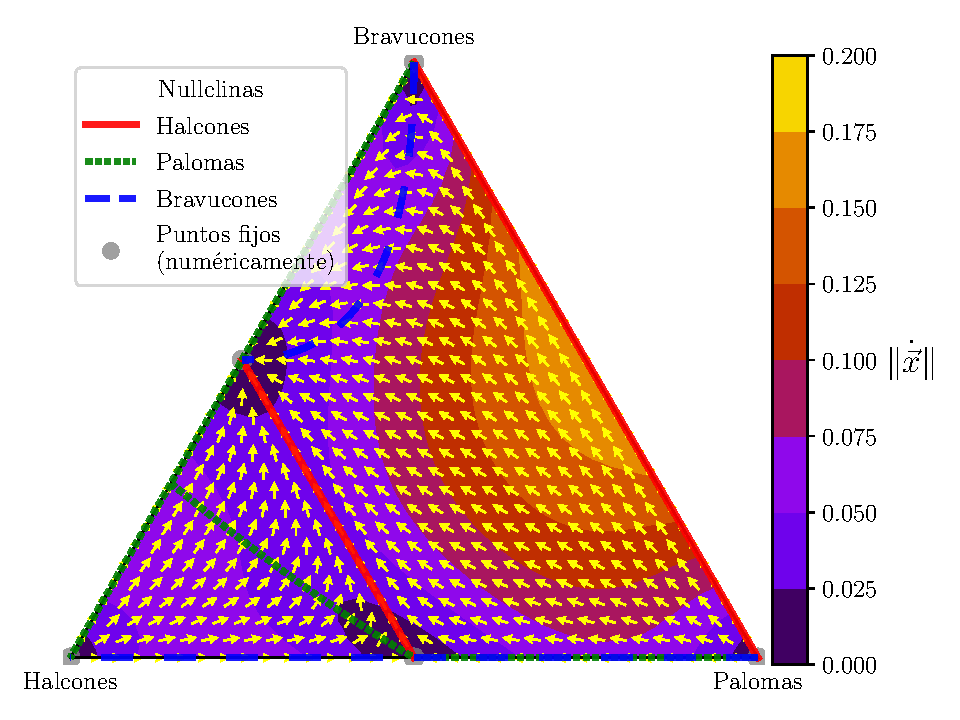
\includegraphics[width = 0.7\textwidth]{figuras/ex01-a.pdf}
        % \caption{}
        % \label{fig:figuras/ex01-a}
    % \end{subfigure}\quad
    \caption{Órbitas en el simplex para el sistema de Halcones, Palomas y Bravucones}
    \label{fig:figuras/ex01-a}
\end{figure*}


Analizando la dinámica del sistema:

$$ \left\lbrace
\begin{aligned}
  \dot{x} &= f_1(x,y,z) = x \left[(A \vec{x})_{x}-\vec{x} \cdot A \vec{x}\right] \\
  \dot{y} &= f_2(x,y,z) = y \left[(A \vec{x})_{y}-\vec{x} \cdot A \vec{x}\right] \\
  \dot{z} &= f_3(x,y,z) = z \left[(A \vec{x})_{z}-\vec{x} \cdot A \vec{x}\right]
\end{aligned}
\right.
$$

Reduciendo a dos variables mediante la condición. $z = 1-x-y$

\sepline

Para el primer sistema y su correspondiente matriz de payoff

$$
Ax = 
\begin{pmatrix}
    \frac{g-c}{2}&g&\frac{g-c}{2}\\
    0&\frac{g}{2}&\frac{g}{2}\\
    \frac{g-c}{2}&\frac{g}{2}&\frac{g}{2}
\end{pmatrix}
\begin{pmatrix}
    x\\
    y\\ 
    1-x-y
\end{pmatrix}
=
\begin{pmatrix}
    \frac{gy+g-c+cy}{2}\\ 
    \frac{g-gx}{2}\\ 
    \frac{g-cx}{2}
\end{pmatrix}
$$

$$(Ax)_x = \frac{gy+g-c+cy}{2}
,\quad 
(Ax)_y = \frac{g-gx}{2}
$$

$$
x^T Ax = \frac{cx^2-2cx+2cxy+g}{2}
$$

$$
f_1(x, y) = 
-x \frac{
    cx^2
    + 2cyx
    - 2cx
    - gy
    - cy
    + c
    }{2}
$$

$$
f_2(x, y) = 
-xy \frac{cx+2cy+g-2c}{2}
$$

% $$
% c((2-(g/c))-2y)^2
% + 2cy((2-(g/c))-2y)
% - 2c((2-(g/c))-2y)
% - gy
% - cy
% + c
% $$

% $$ \left\lbrace
% \begin{aligned}
%   \dot{x} &= x \left[(A \vec{x})_{x}-\vec{x} \cdot A \vec{x}\right] \\
%   \dot{y} &= y \left[(A \vec{x})_{y}-\vec{x} \cdot A \vec{x}\right] \\
%   \dot{z} &= z \left[(A \vec{x})_{z}-\vec{x} \cdot A \vec{x}\right]
% \end{aligned}
% \right.
% $$

Puntos de equilibrio:

\begin{itemize}
    \item[] $P_1^* = (0, \frac{G-2C}{2C}, 1 - \frac{G-2C}{2C})$
    \item[] $P_2^* = (0, 0, 1)$
    \item[] $P_3^* = (0, \frac{C}{G+C}, 1 - \frac{C}{G+C})$
    \item[] $P_4^* = (1, 0, 0)$
    \item[] $P_5^* = (\frac{G}{C}, 1- \frac{G}{C}, 0)$
\end{itemize}

% $$ J =
% \begin{pmatrix}
%     \frac{\partial }{\partial x}\left(-x\frac{cx^2+2cyx-2cx-gy-cy+c}{2}\right) 
%     &
%     \frac{\partial }{\partial y}\left(-x\frac{cx^2+2cyx-2cx-gy-cy+c}{2}\right)
%     \\  
%     \frac{\partial }{\partial x}\left(-xy\frac{cx+2cy+g-2c}{2}\right)          
%     &
%     \frac{\partial }{\partial y}\left(-xy\frac{cx+2cy+g-2c}{2}\right)
% \end{pmatrix}
% $$

% $$J =
% \begin{pmatrix}
%     -\frac{3cx^2-4cx+4cxy+c-gy-cy}{2}
%     &
%     -\frac{x\left(2cx-c-g\right)}{2}
%     \\  
%     -\frac{y\left(2cx-2c+g+2cy\right)}{2}
%     &
%     -\frac{x\left(4cy-2c+g+cx\right)}{2}
% \end{pmatrix}
% $$

% $$J_1 =
% \begin{pmatrix}
%     -\frac{3c(0)^2-4c(0)+4c(0)(\frac{g-2c}{2c})+c-g(\frac{g-2c}{2c})-c(\frac{g-2c}{2c})}{2}
%     &
%     -\frac{(0)\left(2c(0)-c-g\right)}{2}
%     \\  
%     -\frac{(\frac{g-2c}{2c})\left(2c(0)-2c+g+2c(\frac{g-2c}{2c})\right)}{2}
%     &
%     -\frac{(0)\left(4c(\frac{g-2c}{2c})-2c+g+c(0)\right)}{2}
% \end{pmatrix}
% $$

% $$J_1 =
% \begin{pmatrix}
%     -\frac{-g^2+cg+4c^2}{4c}
%     &
%     0
%     \\  
%     -\frac{\left(g-2c\right)^2}{2c}
%     &
%     0
% \end{pmatrix}
% $$


$$J_1 =
\begin{pmatrix}
    -\frac{-g^2+cg+4c^2}{4c}
    &
    0
    \\  
    -\frac{\left(g-2c\right)^2}{2c}
    &
    0
\end{pmatrix}
\Rightarrow \text{Acumulación}
$$


% $$J_2 =
% \begin{pmatrix}
%     -\frac{3c(0)^2-4c(0)+4c(0)(0)+c-g(0)-c(0)}{2}
%     &
%     -\frac{(0)\left(2c(0)-c-g\right)}{2}
%     \\  
%     -\frac{(0)\left(2c(0)-2c+g+2c(0)\right)}{2}
%     &
%     -\frac{(0)\left(4c(0)-2c+g+c(0)\right)}{2}
% \end{pmatrix}
% $$

% $$J_2=
% \begin{pmatrix}
%     -\frac{3c(0)^2-4c(0)+4c(0)(0)+c-g(0)-c(0)}{2}
%     &
%     -\frac{(0)\left(2c(0)-c-g\right)}{2}
%     \\  
%     -\frac{(0)\left(2c(0)-2c+g+2c(0)\right)}{2}
%     &
%     -\frac{(0)\left(4c(0)-2c+g+c(0)\right)}{2}
% \end{pmatrix}
% $$

$$J_2=
\begin{pmatrix}
    -\frac{c}{2}
    &
    0
    \\  
    0
    &
    0
\end{pmatrix}
\Rightarrow \text{Acumulación de estables} 
$$

% $$J_3 =
% \begin{pmatrix}
%     -\frac{3c(0)^2-4c(0)+4c(0)(\frac{c}{g+c})+c-g(\frac{c}{g+c})-c(\frac{c}{g+c})}{2}
%     &
%     -\frac{(0)\left(2c(0)-c-g\right)}{2}
%     \\  
%     -\frac{(\frac{c}{g+c})\left(2c(0)-2c+g+2c(\frac{c}{g+c})\right)}{2}
%     &
%     -\frac{(0)\left(4c(\frac{c}{g+c})-2c+g+c(0)\right)}{2}
% \end{pmatrix}
% $$

$$J_3 =
\begin{pmatrix}
    0
    &
    0
    \\  
    -\frac{c\left(g^2-cg\right)}{2\left(g+c\right)^2}
    &
    0
\end{pmatrix}
\Rightarrow \text{Inconcluso}
$$



% $$J_4 =
% \begin{pmatrix}
%     -\frac{3c(1)^2-4c(1)+4c(1)(0)+c-g(0)-c(0)}{2}
%     &
%     -\frac{(1)\left(2c(1)-c-g\right)}{2}
%     \\  
%     -\frac{(0)\left(2c(1)-2c+g+2c(0)\right)}{2}
%     &
%     -\frac{(1)\left(4c(0)-2c+g+c(1)\right)}{2}
% \end{pmatrix}
% $$

$$J_4 =
\begin{pmatrix}
    0
    &
    -\frac{-g+c}{2}
    \\  
    0
    &
    -\frac{g-c}{2}
\end{pmatrix}
\Rightarrow \text{Acumulación de } ^{\text{Estables si } g>c}_{\text{Inestables si } g<c}
$$

% $$J_5 =
% \begin{pmatrix}
%     -\frac{3c(\frac{g}{c})^2-4c(\frac{g}{c})+4c(\frac{g}{c})(1 - \frac{g}{c})+c-g(1 - \frac{g}{c})-c(1 - \frac{g}{c})}{2}
%     &
%     -\frac{(\frac{g}{c})\left(2c(\frac{g}{c})-c-g\right)}{2}
%     \\  
%     -\frac{(1 - \frac{g}{c})\left(2c(\frac{g}{c})-2c+g+2c(1 - \frac{g}{c})\right)}{2}
%     &
%     -\frac{(\frac{g}{c})\left(4c(1 - \frac{g}{c})-2c+g+c(\frac{g}{c})\right)}{2}
% \end{pmatrix}
% $$

$$J_5 =
\begin{pmatrix}
    0
    &
    -\frac{g\left(g-c\right)}{2c}
    \\  
    -\frac{g\left(-g+c\right)}{2c}
    &
    -\frac{g\left(-g+c\right)}{c}
\end{pmatrix}
\Rightarrow  \lambda_{1,2} = \frac{g}{c} \frac{g-c}{2}
% \Rightarrow \text{Equilibrio }  ^{\text{Estables si } g<c}_{\text{Inestables si } g>c}
$$

$$
\Rightarrow \text{Equilibrio }  ^{\text{Estables si } g<c}_{\text{Inestables si } g>c}
$$

En la Fig. \ref{fig:figuras/ex01-a} se tiene una resolución numérica con $G=1, C=2$.


% ███████╗ ██████╗    ██████╗ 
% ██╔════╝██╔════╝    ╚════██╗
% █████╗  ██║          █████╔╝
% ██╔══╝  ██║         ██╔═══╝ 
% ███████╗╚██████╗    ███████╗
% ╚══════╝ ╚═════╝    ╚══════╝

\sepline

%**********
\begin{figure*}[ht!]
    \centering
    % \begin{subfigure}[b]{0.33\linewidth}
        % \centering
        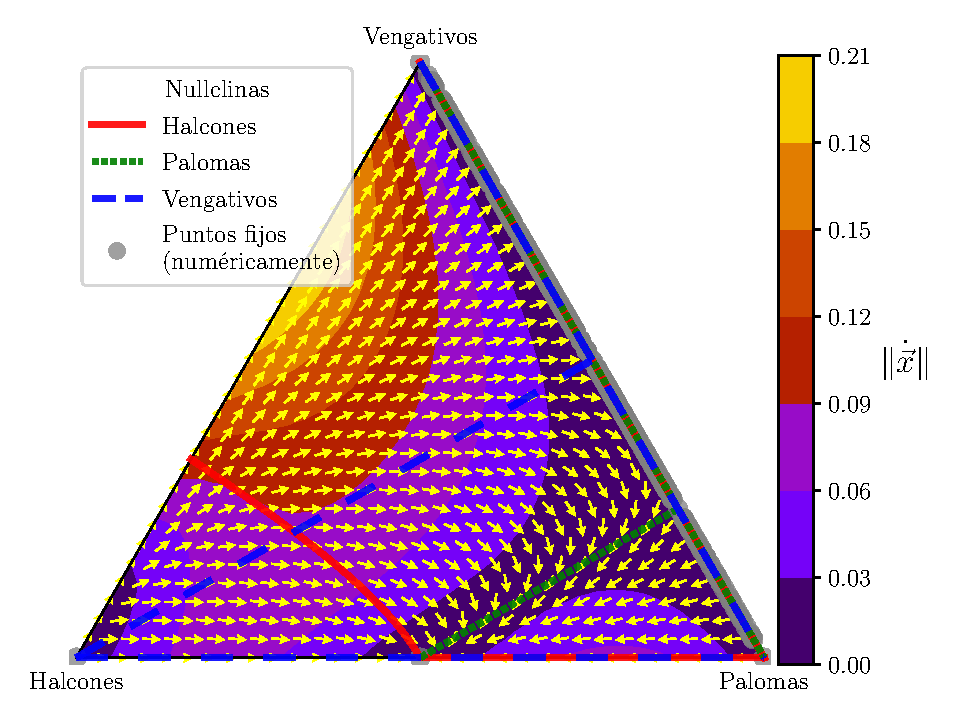
\includegraphics[width = 0.7\textwidth]{figuras/ex01-b.pdf}
        % \caption{}
        % \label{fig:figuras/ex01-b}
    % \end{subfigure}\quad
    \caption{Órbitas en el simplex para el sistema de Halcones, Palomas y vengativos}
    \label{fig:figuras/ex01-b}
\end{figure*}
%**********

Para el segundo sistema

$$
Ax =
\begin{pmatrix}
    \frac{g-c}{2}&g&g\\ 
    0&\frac{g}{2}&0\\ 
    0&g&\frac{g}{2}
\end{pmatrix}
\begin{pmatrix}
    x\\
    y\\ 
    1-x-y
\end{pmatrix}
=
\begin{pmatrix}
    \frac{-gx+2g-cx}{2}\\ 
    \frac{gy}{2}\\ 
    \frac{-gx+gy+g}{2}
\end{pmatrix}
$$


$$
(Ax)_x = \frac{-gx+2g-cx}{2}
, \quad 
(Ax)_y = \frac{gy}{2}
, \quad 
x^T Ax = \frac{g-cx^2}{2}
$$

$$
f_1(x, y) 
% = 
% x
% \frac{-xg+g+cx^2-cx}{2} 
= 
\frac{x}{2} (
    cx^2
    -x(g+c)
    +g
    )
$$

$$
f_2(x, y) 
% = y
% \frac{gy-g+cx^2}{2} 
=
\frac{y}{2} (cx^2+gy-g)
$$

% $$ \left\lbrace
% \begin{aligned}
%   \dot{x} &= x \left[(A \vec{x})_{x}-\vec{x} \cdot A \vec{x}\right] \\
%   \dot{y} &= y \left[(A \vec{x})_{y}-\vec{x} \cdot A \vec{x}\right] \\
%   \dot{z} &= z \left[(A \vec{x})_{z}-\vec{x} \cdot A \vec{x}\right]
% \end{aligned}
% \right.
% $$

Puntos de equilibrio:

\begin{itemize}
    \item[] $P_1^* = (0, 0, 1 )$
    \item[] $P_2^* = (0, 1, 0)$
    \item[] $P_3^* = (1, 0, 0)$
    \item[] $P_4^* = (\frac{G}{C}, 0, 1- \frac{G}{C})$
\end{itemize}

% $$ J =
% \begin{pmatrix}
%     \frac{\partial }{\partial x}\left(\frac{x}{2} (cx^2-x(g+c)+g)\right)
%     &
%     \frac{\partial }{\partial y}\left(\frac{x}{2} (cx^2-x(g+c)+g)\right)
%     \\  
%     \frac{\partial }{\partial x}\left(\frac{y}{2} (cx^2+gy-g)\right)          
%     &
%     \frac{\partial }{\partial y}\left(\frac{y}{2} (cx^2+gy-g)\right)
% \end{pmatrix}
% $$

% $$ J =
% \begin{pmatrix}
%     \frac{3x^2c-2xc-2xg+g}{2}
%     &
%     0
%     \\  
%     cyx
%     &
%     \frac{2gy-g+cx^2}{2}
% \end{pmatrix}
% $$

$$ J_1 =
\begin{pmatrix}
    \frac{g}{2}
    &
    0
    \\  
    0
    &
    -\frac{g}{2}
\end{pmatrix}
\Rightarrow Saddle
$$

$$ J_2 =
\begin{pmatrix}
    \frac{g}{2}
    &
    0
    \\  
    0
    &
    \frac{g}{2}
\end{pmatrix}
\Rightarrow \text{Inestable}
$$

$$ J_3 =
\begin{pmatrix}
    \frac{c-g}{2}
    &
    0
    \\  
    0
    &
    \frac{c-g}{2}
\end{pmatrix}
\Rightarrow \text{Equilibrio }  ^{\text{Estables si } g>c}_{\text{Inestables si } g<c}
$$

$$ J_4 =
\begin{pmatrix}
    \frac{g}{c} \frac{g-c}{2}
    &
    0
    \\  
    0
    &
    \frac{g}{c} \frac{g-c}{2}
\end{pmatrix}
\Rightarrow \text{Equilibrio }  ^{\text{Estables si } g<c}_{\text{Inestables si } g>c}
$$

En la Fig. \ref{fig:figuras/ex01-b} se tiene una resolución numérica con $G=1, C=2$.

\section{Resolución Ej 2}
% ███████╗██╗  ██╗    ██████╗  
% ██╔════╝╚██╗██╔╝    ╚════██╗
% █████╗   ╚███╔╝      █████╔╝
% ██╔══╝   ██╔██╗     ██╔═══╝ 
% ███████╗██╔╝ ██╗    ███████╗
% ╚══════╝╚═╝  ╚═╝    ╚══════╝

\textbf{Dilema del prisionero un jugador:}

% \begin{table}[!ht]
%     \begin{tabular}{c|ccccc}
%     Jugadores & 0       & 1        \\ \hline
%     $C$       & $C_{0}$ & $C_{1}$  \\ \hline
%     $D$       & $D_{0}$ & $D_{1}$ 
%     \end{tabular}
%     \caption{Payoff de las estrategias $C$ y $D$ cuando compiten con $m$ cooperadores y $n-m$ defectores, para un total de $n$ jugadores.}
%     \label{tab:my-table}
% \end{table}

\begin{table}[!htb]
    \begin{subtable}{.5\linewidth}
      \centering
        \caption{}
        \begin{tabular}{c|ccccc}
            Jugadores & 0       & 1        \\ \hline
            $C$       & $C_{0}$ & $C_{1}$  \\ \hline
            $D$       & $D_{0}$ & $D_{1}$ 
            \end{tabular}
            % \caption{Payoff de las estrategias $C$ y $D$ cuando compiten con $m$ cooperadores y $n-m$ defectores, para un total de $n$ jugadores.}
            \label{tab:my-table}
    \end{subtable}%
    \begin{subtable}{.5\linewidth}
      \centering
        \caption{}
        \begin{tabular}{c|ccccc}
            Jugadores & 0       & 1        \\ \hline
            $C$       & $S$ & $R$  \\ \hline
            $D$       & $P$ & $T$ 
            \end{tabular}
        \end{subtable} 
    \caption{Payoff de las estrategias $C$ y $D$ cuando compiten dos jugadores.}
    \label{tab:my-table}
\end{table}

El dilema de dos jugadores viene dado por:

$$
\begin{aligned}
    T &= \text{ Tentación para defraudar}\\
    R &= \text{ Recompensa por cooperar}\\
    P &= \text{ Penalidad por defraudar mutuamente}\\
    S &= \text{ Sucker's payoff},
\end{aligned}
$$

resultando

$$
T > R > P > S
$$

Para 2 jugadores:

\begin{itemize}
    \item Defraudar cuando uno coopera ofrece el mayor payoff $T$.
    \item Cooperar cuando uno coopera ofrece el segundo mejor payoff $R$.
    \item Defraudar cuando nadie coopera ofrece el segundo peor payoff $P$.
    \item Cooperar cuando nadie coopera ofrece el peor payoff $S$.
\end{itemize}

\textbf{Dilema del prisionero multijugador:}

Para el caso multijugador se considera:

\begin{itemize}
    \item $C_i$: Payoff si cooperan $i$ jugadores y coopero.
    \item $D_i$: Payoff si cooperan $i$ jugadores y defraudo.
\end{itemize}

Con esto en cuenta para $n=2$ jugadores se tiene:

$$
D_1 > C_1 > D_0 > C_0
$$

Extendiendo esto para mas jugadores:

\begin{itemize}
    \item Defraudar cuando todos cooperan ofrece el mayor payoff $T$.
    \item Cooperar cuando uno coopera ofrece el segundo mejor payoff $R$.
    \item Defraudar cuando nadie coopera ofrece el segundo peor payoff $P$.
    \item Cooperar cuando nadie cooperan ofrece el peor payoff $S$.
\end{itemize}

$$
  \underbrace{D_{n-1 }}_{T} 
> \underbrace{C_{n-1 }}_{R} 
> \underbrace{\ldots}_{\text{El resto de payoffs}} 
> \underbrace{D_{0 }}_{P}
> \underbrace{C_{0 }}_{S}
$$

Uno podría detenerse en este punto, con el resto de payoffs en un orden arbitrario. Pero, si deseo que cada subconjunto de jugadores tengan un dilema del prisionero con reglas similares uno podría tomar caso de $n$ jugadores como una extensión del caso $n-1$ jugadores, arrancando desde dos jugadores. Algo como:

$$
\begin{aligned}
  D_{1 }   > C_{1 }   > D_{0 }   &> C_{0 }    \\
  D_{2 }   > C_{2 }   > D_{1 }   > C_{1 }   > D_{0 } &> C_{0 }  \\
  D_{3 }   > C_{3 }   > D_{2 }   > C_{2 }   > D_{1 } > C_{1 } > D_{0 } &> C_{0 }  \\
  D_{n-1 } > C_{n-1 } > D_{n-2 } > C_{n-2 } > \ldots > D_{1 } > C_{1 } > D_{0 } &> C_{0 }\\
\end{aligned}
$$

Es decir $D_i > C_i, \forall i = 1, 2, ..., n-1$. 

% \bibliography{sample}

\end{document}